% Questions on PDF page 134
\documentclass[12pt]{article}

\usepackage[utf8]{inputenc}
\usepackage[a4paper, margin=1in]{geometry}
\usepackage{booktabs}
\usepackage{enumerate}
\usepackage{physics}
\usepackage{amsmath}
\usepackage{amsfonts}
\usepackage{graphicx}
\usepackage{siunitx}
\usepackage{textcomp}
\usepackage{hyperref}

\bibliographystyle{ieeetr}
\graphicspath{{./figures}}

\title{Big Data (AES 630) Homework 2}
\author{Mitchell Dodson}
\date{February 8, 2024}

\newcommand*{\problem}[2]{
    \begin{table}[ht]
    \centering
        \begin{tabular}{ | p{.1\linewidth} p{.9\linewidth} | }
            \hline
            \vspace{.3em}\textbf{\large#1:} & \vspace{.3em}\small{#2}\hspace{.2em}\vspace{.5em} \\ \hline
        \end{tabular}
    \end{table}
}

\begin{document}

\maketitle

\section{Data compression}

The dataset I will be using for this assignment is an 8-dimensional lookup table for spectral flux with respect to multiple atmospheric profiles, cloud properties, and solar angles. The table is dimensionally organized like (`idatm', `zcloud', `tcloud', `nre', `sza', `wl', `z', `flux') and has shape ().

I chose to use the lookup table out of curiosity for how the compression would respond to the table's high dimensionality and redundancy across some axes. The table was generated using a generalized python wrapper I made for the SBDART radiative transfer model, which is available on my github: \url{https://github.com/Mitchell-D/quickrad}

\begin{figure}[h!]
    \centering
    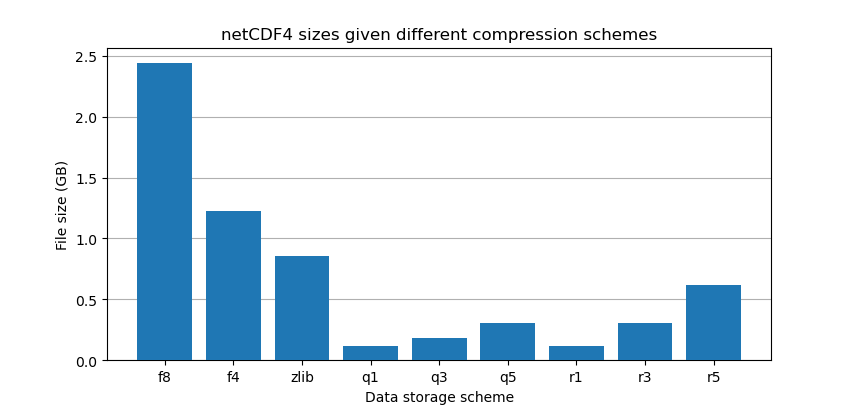
\includegraphics[width=.8\paperwidth]{figs/sizes.png}
    \caption{File sizes after compression using different methods. `f4' and `f8' represent 32-bit and 64-bit floats, respectively, r1-r5 represents 64 bit float values rounded to the 1st-5th decimals, and q1-q5 represents 64 bit float values quantized to the 1st-5th significant digits. Each of the results were subsequently compressed using zlib for comparison.}
    \label{sizes}
\end{figure}

Figure \ref{sizes} shows the file sizes and compression ratios of the dataset after compression by data type reduction, value rounding, and significant digit quantization.

\begin{figure}[h!]
    \centering
    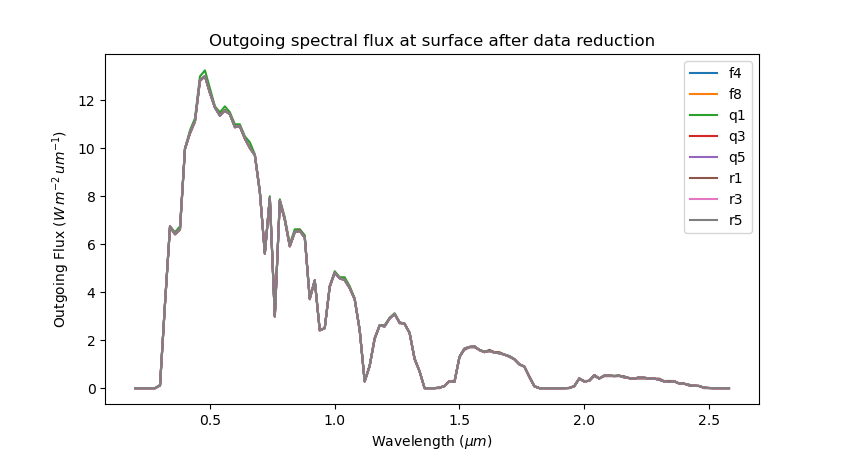
\includegraphics[width=.8\paperwidth]{figs/sflux.png}

    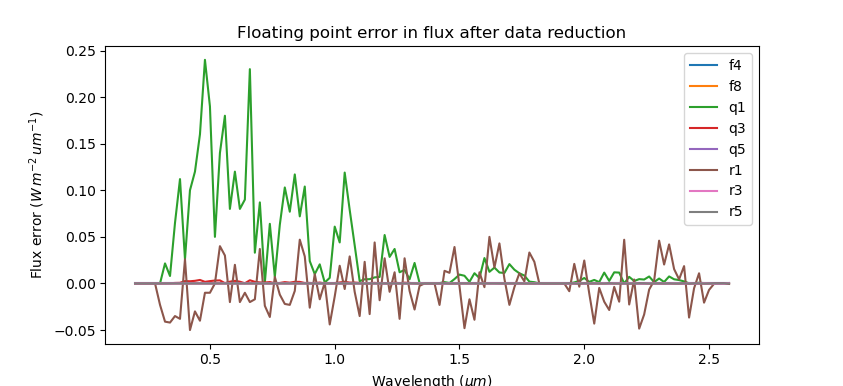
\includegraphics[width=.8\paperwidth]{figs/error.png}
    \caption{Outgoing radiative flux at the surface wrt wavelength, and floating point error rate wrt wavelength given each of the compression schemes. Data are extracted by assuming outgoing flux measurements were taken at the surface at noon with a tropical atmosphere, and a water cloud at $1\,\si{km}$ having optical depth $\tau=0.01$ and effective particle size $r=20\,\si{\mu m}$.}
    \label{sflux}
\end{figure}

Figure \ref{sflux} shows the value difference in outgoing radiation between a small subset of values in the table.

\section{Cloud data access}

The version of GMGSI data hosted on the AWS bucket is stored as integers in the range $[0,255]$. I used s3fs and \texttt{xarray.open\_mfdataset} to load all the hourly files from the UTC day of January 15, 2024, then restricted the domain to only include SEUS pixels using boolean masks derived from the thresholds $lat \in [25,35]$ and $lon \in [-95,-75]$.

\end{document}

\begin{figure}[h!]\label{q1q2}
    \centering
    \begin{tabular}{ c c c | c}
    \end{tabular}
\end{figure}

